\section{Penerapan Aljabar Boolean dalam Rangkaian Digital}

Aljabar Boolean memperoleh relevansi praktis yang besar melalui penerapannya dalam perancangan rangkaian digital. Setiap ekspresi aljabar Boolean dapat direalisasikan secara langsung sebagai rangkaian gerbang logika elektronik, dan sebaliknya, setiap rangkaian gerbang logika dapat dianalisis dan disederhanakan menggunakan aljabar Boolean. Hubungan langsung antara representasi matematis dan implementasi fisik ini menjadikan aljabar Boolean sebagai bahasa universal dalam teknik desain digital \cite{grinnell_logic}.

\subsection{Gerbang Logika Dasar}

Gerbang logika (\textit{logic gate}) adalah komponen elektronik dasar yang mengimplementasikan operasi aljabar Boolean. Setiap gerbang menerima satu atau lebih sinyal input biner dan menghasilkan satu sinyal output biner berdasarkan fungsi Boolean yang didefinisikan untuknya. Terdapat enam jenis gerbang logika yang paling umum digunakan, sebagaimana dirangkum pada Tabel~\ref{tab:gerbang-logika} \cite{hackatronic}.

\begin{table}[H]
\centering
\small
\renewcommand{\arraystretch}{1.3}
\begin{tabular}{|l|c|>{\raggedright\arraybackslash}p{4.5cm}|c|}
\hline
\textbf{Gerbang} & \textbf{Ekspresi} & \textbf{Deskripsi} & \textbf{Jumlah Input} \\ \hline
AND & $F = x \cdot y$ & Output 1 jika semua input 1 & $\geq 2$ \\ \hline
OR & $F = x + y$ & Output 1 jika salah satu input 1 & $\geq 2$ \\ \hline
NOT & $F = x'$ & Membalikkan nilai input & 1 \\ \hline
NAND & $F = (x \cdot y)'$ & NOT-AND, output 0 hanya jika semua input 1 & $\geq 2$ \\ \hline
NOR & $F = (x + y)'$ & NOT-OR, output 1 hanya jika semua input 0 & $\geq 2$ \\ \hline
XOR & $F = x \oplus y$ & Output 1 jika jumlah input bernilai 1 ganjil (untuk 2 input: tepat satu input bernilai 1) & 2 \\ \hline
\end{tabular}
\caption{Jenis-Jenis Gerbang Logika dan Ekspresi Booleannya}
\label{tab:gerbang-logika}
\end{table}

Gambar~\ref{fig:gerbang-dasar} menampilkan simbol standar berdasarkan standar IEEE/ANSI untuk ketiga gerbang logika dasar (AND, OR, NOT) beserta tabel kebenarannya.

\begin{figure}[H]
\centering
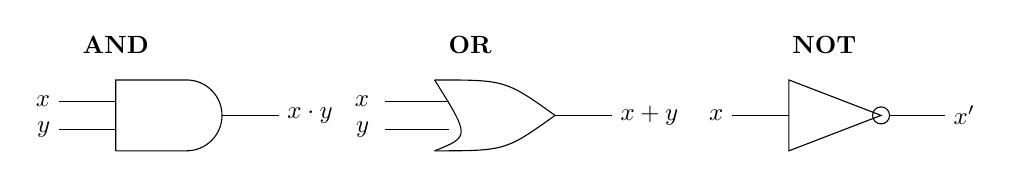
\begin{tikzpicture}[scale=0.9, transform shape]
  % --- AND Gate ---
  \node at (0, 3) {\textbf{AND}};
  \draw (0, 1.5) -- (0, 2.5) -- (1, 2.5) arc (90:-90:0.5) -- (0, 1.5);
  \draw (-0.8, 2.2) -- (0, 2.2) node[left, xshift=-0.8cm] {$x$};
  \draw (-0.8, 1.8) -- (0, 1.8) node[left, xshift=-0.8cm] {$y$};
  \draw (1.5, 2) -- (2.3, 2) node[right] {$x \cdot y$};

  % --- OR Gate ---
  \node at (5, 3) {\textbf{OR}};
  \draw (4.5, 1.5) .. controls (5,1.7) .. (4.5, 2.5);
  \draw (4.5, 2.5) .. controls (5.5,2.5) .. (6.2, 2);
  \draw (4.5, 1.5) .. controls (5.5,1.5) .. (6.2, 2);
  \draw (3.8, 2.2) -- (4.7, 2.2) node[left, xshift=-1cm] {$x$};
  \draw (3.8, 1.8) -- (4.7, 1.8) node[left, xshift=-1cm] {$y$};
  \draw (6.2, 2) -- (7, 2) node[right] {$x + y$};

  % --- NOT Gate ---
  \node at (10, 3) {\textbf{NOT}};
  \draw (9.5, 1.5) -- (9.5, 2.5) -- (10.8, 2) -- cycle;
  \draw (10.8, 2) circle (0.12);
  \draw (8.7, 2) -- (9.5, 2) node[left, xshift=-0.8cm] {$x$};
  \draw (10.92, 2) -- (11.7, 2) node[right] {$x'$};
\end{tikzpicture}
\caption{Simbol Gerbang Logika Dasar: AND, OR, dan NOT}
\label{fig:gerbang-dasar}
\end{figure}

\subsection{Kelengkapan Fungsional (Functional Completeness)}

Suatu himpunan operator Boolean dikatakan \logic{lengkap secara fungsional} (\textit{functionally complete}) jika setiap fungsi Boolean dapat diekspresikan hanya dengan menggunakan operator-operator dalam himpunan tersebut. Himpunan $\{AND, OR, NOT\}$ jelas bersifat lengkap secara fungsional karena setiap fungsi Boolean dapat ditulis dalam bentuk SOP yang hanya menggunakan ketiga operator tersebut \cite{rosen2019}.

Namun hasil yang lebih mengejutkan adalah bahwa gerbang NAND dan gerbang NOR masing-masing secara individual bersifat lengkap secara fungsional. Sifat kelengkapan fungsional NAND (dan NOR) pertama kali dibuktikan oleh Henry M. Sheffer pada tahun 1913. Artinya, seluruh rangkaian digital apa pun dapat dibangun hanya menggunakan satu jenis gerbang (NAND saja atau NOR saja). Hal ini dibuktikan dengan menunjukkan bahwa ketiga operator dasar dapat diimplementasikan hanya menggunakan NAND:

\begin{align*}
\text{NOT: } x' &= (x \cdot x)' = x \uparrow x \\
\text{AND: } x \cdot y &= ((x \cdot y)')' = (x \uparrow y) \uparrow (x \uparrow y) \\
\text{OR: } x + y &= (x' \cdot y')' = (x \uparrow x) \uparrow (y \uparrow y)
\end{align*}

Properti ini memiliki implikasi praktis yang signifikan karena dalam fabrikasi chip semikonduktor, memproduksi satu jenis gerbang secara massal lebih efisien daripada memproduksi beragam jenis gerbang. Oleh karena itu, banyak keluarga logika digital, seperti TTL (Transistor-Transistor Logic), menggunakan gerbang NAND sebagai komponen dasar \cite{allaboutcircuits_gates}.

\subsection{Dari Ekspresi Boolean ke Rangkaian Gerbang}

Proses konversi dari ekspresi aljabar Boolean ke rangkaian gerbang logika bersifat mekanistik dan langsung. Setiap operasi AND dalam ekspresi diterjemahkan menjadi gerbang AND, setiap operasi OR menjadi gerbang OR, dan setiap komplemen menjadi gerbang NOT. Interkoneksi antar gerbang mengikuti struktur ekspresi.

\begin{contoh}
\textbf{Implementasi Rangkaian untuk $F = xy + x'z$}

Ekspresi $F = xy + x'z$ memerlukan:
\begin{itemize}
    \item 1 gerbang NOT (untuk menghasilkan $x'$)
    \item 2 gerbang AND (untuk menghasilkan $xy$ dan $x'z$)
    \item 1 gerbang OR (untuk menjumlahkan kedua suku)
\end{itemize}

Total: 4 gerbang logika. Jika ekspresi ini dapat disederhanakan lebih lanjut (pada kasus ini tidak), jumlah gerbang yang diperlukan akan berkurang.
\end{contoh}

\subsection{Studi Kasus: Rangkaian Voting Mayoritas 3-Input}

\begin{contoh}
\textbf{Perancangan Rangkaian Voting Mayoritas}

Sebuah sistem voting elektronik sederhana memiliki tiga pemilih ($A$, $B$, $C$). Keputusan diambil berdasarkan suara mayoritas: output $F = 1$ jika minimal 2 dari 3 pemilih memberikan suara setuju ($= 1$).

\textbf{Langkah 1: Buat Tabel Kebenaran}

\begin{center}
\begin{tabular}{|c|c|c||c|l|}
\hline
$A$ & $B$ & $C$ & $F$ & \textbf{Keterangan} \\ \hline
0 & 0 & 0 & 0 & 0 suara setuju \\ \hline
0 & 0 & 1 & 0 & 1 suara setuju \\ \hline
0 & 1 & 0 & 0 & 1 suara setuju \\ \hline
0 & 1 & 1 & 1 & 2 suara setuju ($\geq$ mayoritas) \\ \hline
1 & 0 & 0 & 0 & 1 suara setuju \\ \hline
1 & 0 & 1 & 1 & 2 suara setuju ($\geq$ mayoritas) \\ \hline
1 & 1 & 0 & 1 & 2 suara setuju ($\geq$ mayoritas) \\ \hline
1 & 1 & 1 & 1 & 3 suara setuju ($\geq$ mayoritas) \\ \hline
\end{tabular}
\end{center}

\textbf{Langkah 2: Bentuk Kanonik SOP}
\[ F = \sum m(3, 5, 6, 7) = A'BC + AB'C + ABC' + ABC \]

\textbf{Langkah 3: Sederhanakan}
\begin{align*}
F &= A'BC + AB'C + ABC' + ABC \\
  &= A'BC + ABC + AB'C + ABC + ABC' + ABC & \text{(Idempoten)} \\
  &= BC(A' + A) + AC(B' + B) + AB(C' + C) & \text{(Distributif)} \\
  &= BC \cdot 1 + AC \cdot 1 + AB \cdot 1 & \text{(Komplemen)} \\
  &= AB + AC + BC & \text{(Identitas)}
\end{align*}

\textbf{Langkah 4: Hitung Kebutuhan Gerbang}

Ekspresi terakhir $F = AB + AC + BC$ memerlukan:
\begin{itemize}
    \item 3 gerbang AND (2-input masing-masing)
    \item 1 gerbang OR (3-input)
\end{itemize}
Total: 4 gerbang, jauh lebih sedikit dibandingkan 10+ gerbang yang dibutuhkan oleh bentuk kanonik SOP awalnya.
\end{contoh}

\subsection{Pengantar ke Bab Selanjutnya}

Meskipun metode penyederhanaan aljabar yang telah dibahas dalam bab ini sangat berguna, metode ini memiliki keterbatasan. Pertama, tidak terdapat algoritma sistematis yang menjamin bahwa solusi yang diperoleh adalah solusi optimal (paling sederhana). Kedua, untuk fungsi dengan banyak variabel dan banyak suku, proses penyederhanaan aljabar menjadi rumit dan rentan terhadap kesalahan manusia. Ketiga, kemampuan untuk ``melihat'' penyederhanaan yang tepat seringkali bergantung pada pengalaman dan intuisi perancang \cite{allaboutcircuits_boolean}.

Pada Bab~10, akan diperkenalkan \logic{Peta Karnaugh} (K-Map), sebuah metode grafis yang memberikan prosedur penyederhanaan yang lebih sistematik dan visual. Peta Karnaugh memungkinkan perancang mengidentifikasi peluang penyederhanaan melalui pengenalan pola pada peta dua dimensi, sehingga mengurangi ketergantungan pada manipulasi aljabar yang rumit. Metode ini efektif untuk fungsi hingga 4--6 variabel dan menjadi pendahulu metode algoritmik seperti algoritma Quine--McCluskey untuk fungsi dengan variabel yang lebih banyak \cite{wiki_karnaugh}.
